% Options for packages loaded elsewhere
\PassOptionsToPackage{unicode}{hyperref}
\PassOptionsToPackage{hyphens}{url}
%
\documentclass[
]{article}
\usepackage{amsmath,amssymb}
\usepackage{lmodern}
\usepackage{iftex}
\ifPDFTeX
  \usepackage[T1]{fontenc}
  \usepackage[utf8]{inputenc}
  \usepackage{textcomp} % provide euro and other symbols
\else % if luatex or xetex
  \usepackage{unicode-math}
  \defaultfontfeatures{Scale=MatchLowercase}
  \defaultfontfeatures[\rmfamily]{Ligatures=TeX,Scale=1}
\fi
% Use upquote if available, for straight quotes in verbatim environments
\IfFileExists{upquote.sty}{\usepackage{upquote}}{}
\IfFileExists{microtype.sty}{% use microtype if available
  \usepackage[]{microtype}
  \UseMicrotypeSet[protrusion]{basicmath} % disable protrusion for tt fonts
}{}
\makeatletter
\@ifundefined{KOMAClassName}{% if non-KOMA class
  \IfFileExists{parskip.sty}{%
    \usepackage{parskip}
  }{% else
    \setlength{\parindent}{0pt}
    \setlength{\parskip}{6pt plus 2pt minus 1pt}}
}{% if KOMA class
  \KOMAoptions{parskip=half}}
\makeatother
\usepackage{xcolor}
\IfFileExists{xurl.sty}{\usepackage{xurl}}{} % add URL line breaks if available
\IfFileExists{bookmark.sty}{\usepackage{bookmark}}{\usepackage{hyperref}}
\hypersetup{
  pdftitle={SICP Chapter 1},
  pdfauthor={ProducerMatt},
  hidelinks,
  pdfcreator={LaTeX via pandoc}}
\urlstyle{same} % disable monospaced font for URLs
\usepackage{color}
\usepackage{fancyvrb}
\newcommand{\VerbBar}{|}
\newcommand{\VERB}{\Verb[commandchars=\\\{\}]}
\DefineVerbatimEnvironment{Highlighting}{Verbatim}{commandchars=\\\{\}}
% Add ',fontsize=\small' for more characters per line
\newenvironment{Shaded}{}{}
\newcommand{\AlertTok}[1]{\textcolor[rgb]{1.00,0.00,0.00}{\textbf{#1}}}
\newcommand{\AnnotationTok}[1]{\textcolor[rgb]{0.38,0.63,0.69}{\textbf{\textit{#1}}}}
\newcommand{\AttributeTok}[1]{\textcolor[rgb]{0.49,0.56,0.16}{#1}}
\newcommand{\BaseNTok}[1]{\textcolor[rgb]{0.25,0.63,0.44}{#1}}
\newcommand{\BuiltInTok}[1]{#1}
\newcommand{\CharTok}[1]{\textcolor[rgb]{0.25,0.44,0.63}{#1}}
\newcommand{\CommentTok}[1]{\textcolor[rgb]{0.38,0.63,0.69}{\textit{#1}}}
\newcommand{\CommentVarTok}[1]{\textcolor[rgb]{0.38,0.63,0.69}{\textbf{\textit{#1}}}}
\newcommand{\ConstantTok}[1]{\textcolor[rgb]{0.53,0.00,0.00}{#1}}
\newcommand{\ControlFlowTok}[1]{\textcolor[rgb]{0.00,0.44,0.13}{\textbf{#1}}}
\newcommand{\DataTypeTok}[1]{\textcolor[rgb]{0.56,0.13,0.00}{#1}}
\newcommand{\DecValTok}[1]{\textcolor[rgb]{0.25,0.63,0.44}{#1}}
\newcommand{\DocumentationTok}[1]{\textcolor[rgb]{0.73,0.13,0.13}{\textit{#1}}}
\newcommand{\ErrorTok}[1]{\textcolor[rgb]{1.00,0.00,0.00}{\textbf{#1}}}
\newcommand{\ExtensionTok}[1]{#1}
\newcommand{\FloatTok}[1]{\textcolor[rgb]{0.25,0.63,0.44}{#1}}
\newcommand{\FunctionTok}[1]{\textcolor[rgb]{0.02,0.16,0.49}{#1}}
\newcommand{\ImportTok}[1]{#1}
\newcommand{\InformationTok}[1]{\textcolor[rgb]{0.38,0.63,0.69}{\textbf{\textit{#1}}}}
\newcommand{\KeywordTok}[1]{\textcolor[rgb]{0.00,0.44,0.13}{\textbf{#1}}}
\newcommand{\NormalTok}[1]{#1}
\newcommand{\OperatorTok}[1]{\textcolor[rgb]{0.40,0.40,0.40}{#1}}
\newcommand{\OtherTok}[1]{\textcolor[rgb]{0.00,0.44,0.13}{#1}}
\newcommand{\PreprocessorTok}[1]{\textcolor[rgb]{0.74,0.48,0.00}{#1}}
\newcommand{\RegionMarkerTok}[1]{#1}
\newcommand{\SpecialCharTok}[1]{\textcolor[rgb]{0.25,0.44,0.63}{#1}}
\newcommand{\SpecialStringTok}[1]{\textcolor[rgb]{0.73,0.40,0.53}{#1}}
\newcommand{\StringTok}[1]{\textcolor[rgb]{0.25,0.44,0.63}{#1}}
\newcommand{\VariableTok}[1]{\textcolor[rgb]{0.10,0.09,0.49}{#1}}
\newcommand{\VerbatimStringTok}[1]{\textcolor[rgb]{0.25,0.44,0.63}{#1}}
\newcommand{\WarningTok}[1]{\textcolor[rgb]{0.38,0.63,0.69}{\textbf{\textit{#1}}}}
\usepackage{longtable,booktabs,array}
\usepackage{calc} % for calculating minipage widths
% Correct order of tables after \paragraph or \subparagraph
\usepackage{etoolbox}
\makeatletter
\patchcmd\longtable{\par}{\if@noskipsec\mbox{}\fi\par}{}{}
\makeatother
% Allow footnotes in longtable head/foot
\IfFileExists{footnotehyper.sty}{\usepackage{footnotehyper}}{\usepackage{footnote}}
\makesavenoteenv{longtable}
\usepackage{graphicx}
\makeatletter
\def\maxwidth{\ifdim\Gin@nat@width>\linewidth\linewidth\else\Gin@nat@width\fi}
\def\maxheight{\ifdim\Gin@nat@height>\textheight\textheight\else\Gin@nat@height\fi}
\makeatother
% Scale images if necessary, so that they will not overflow the page
% margins by default, and it is still possible to overwrite the defaults
% using explicit options in \includegraphics[width, height, ...]{}
\setkeys{Gin}{width=\maxwidth,height=\maxheight,keepaspectratio}
% Set default figure placement to htbp
\makeatletter
\def\fps@figure{htbp}
\makeatother
\setlength{\emergencystretch}{3em} % prevent overfull lines
\providecommand{\tightlist}{%
  \setlength{\itemsep}{0pt}\setlength{\parskip}{0pt}}
\setcounter{secnumdepth}{-\maxdimen} % remove section numbering
\setmonofont[Mapping=tex-text,Scale=MatchLowercase]{FiraMono-Regular}
\listfiles
\ifLuaTeX
  \usepackage{selnolig}  % disable illegal ligatures
\fi

\title{SICP Chapter 1}
\author{ProducerMatt}
\date{}

\begin{document}
\maketitle

\hypertarget{how-this-document-is-made}{%
\section{HOW THIS DOCUMENT IS MADE}\label{how-this-document-is-made}}

\textbf{\textbf{TODO}}

\hypertarget{testing}{%
\label{testing}}%
\begin{Shaded}
\begin{Highlighting}[numbers=left,,]
\NormalTok{(}\ExtensionTok{define}\FunctionTok{ }\NormalTok{(foo a b)}
\NormalTok{  (}\OperatorTok{+}\NormalTok{ a (}\OperatorTok{*} \DecValTok{2}\NormalTok{ b)))}

\NormalTok{(foo }\DecValTok{5} \DecValTok{3}\NormalTok{)}
\end{Highlighting}
\end{Shaded}

11

\^{} Dynamically evaluated when you press "enter" on the
\texttt{BEGIN\_SRC} block!

\hypertarget{also-consider}{%
\subsubsection{Also consider:}\label{also-consider}}

\begin{itemize}
\tightlist
\item
  \texttt{:results\ output} for what the code prints
\item
  \texttt{:exports\ code} or \texttt{:exports\ results} to just get one
  or the other
\end{itemize}

\(a + (\pi \times b)\) \textless\textasciitilde{} inline Latex btw :)

\hypertarget{current-command-for-conversion}{%
\subsubsection{Current command for
conversion}\label{current-command-for-conversion}}

\begin{Shaded}
\begin{Highlighting}[]
\ExtensionTok{pandoc} \AttributeTok{{-}{-}from}\NormalTok{ org }\AttributeTok{{-}{-}to}\NormalTok{ latex 1.org }\AttributeTok{{-}o}\NormalTok{ 1.tex }\AttributeTok{{-}s}\KeywordTok{;} \ExtensionTok{xelatex}\NormalTok{ 1.tex}
\end{Highlighting}
\end{Shaded}

\hypertarget{helpers-for-org-mode-tables}{%
\subsection{Helpers for org-mode
tables}\label{helpers-for-org-mode-tables}}

\hypertarget{try-these}{%
\subsubsection{\texorpdfstring{\texttt{try-these}}{try-these}}\label{try-these}}

Takes function \texttt{f} and list \texttt{testvals} and applies
\texttt{f} to each item \texttt{i}. For each \texttt{i} returns a list
with \texttt{i} and the result. Useful dor making tables with a column
for input and a column for output.

\hypertarget{try-these}{%
\label{try-these}}%
\begin{Shaded}
\begin{Highlighting}[numbers=left,,]
\CommentTok{;; Surely this could be less nightmarish}
\NormalTok{(}\ExtensionTok{define}\FunctionTok{ }\NormalTok{(try{-}these f }\OperatorTok{.}\NormalTok{ testvals)}
\NormalTok{  (}\KeywordTok{let}\NormalTok{ ((l (}\KeywordTok{if}\NormalTok{ (}\KeywordTok{and}\NormalTok{ (}\OperatorTok{=} \DecValTok{1}\NormalTok{ (}\KeywordTok{length}\NormalTok{ testvals))}
\NormalTok{                    (}\KeywordTok{list?}\NormalTok{ (}\KeywordTok{car}\NormalTok{ testvals)))}
\NormalTok{               (}\KeywordTok{car}\NormalTok{ testvals)}
\NormalTok{               testvals)))}
\NormalTok{    (map (λ (i) (}\KeywordTok{cons}\NormalTok{ i}
\NormalTok{                      (}\KeywordTok{cons}\NormalTok{ (}\KeywordTok{if}\NormalTok{ (}\KeywordTok{list?}\NormalTok{ i)}
\NormalTok{                                (apply f i)}
\NormalTok{                                (f i))}
\NormalTok{                            \#nil)))}
\NormalTok{         l)))}
\end{Highlighting}
\end{Shaded}

\hypertarget{transpose-list}{%
\subsubsection{\texorpdfstring{\texttt{transpose-list}}{transpose-list}}\label{transpose-list}}

"Rotate" a list, for example from
\VERB|\NormalTok{\textquotesingle{}(}\DecValTok{1} \DecValTok{2} \DecValTok{3}\NormalTok{)}|
to
\VERB|\NormalTok{\textquotesingle{}(\textquotesingle{}(}\DecValTok{1}\NormalTok{) \textquotesingle{}(}\DecValTok{2}\NormalTok{) \textquotesingle{}(}\DecValTok{3}\NormalTok{))}|

\hypertarget{transpose-list}{%
\label{transpose-list}}%
\begin{Shaded}
\begin{Highlighting}[numbers=left,,]
\NormalTok{(}\ExtensionTok{define}\FunctionTok{ }\NormalTok{(transpose{-}list l)}
\NormalTok{  (map (λ (i) (}\KeywordTok{list}\NormalTok{ i)) l))}
\end{Highlighting}
\end{Shaded}

\hypertarget{print-as-rows}{%
\subsubsection{\texorpdfstring{\texttt{print-as-rows}}{print-as-rows}}\label{print-as-rows}}

For manually printing items in rows to stdout. Not currently used.

\hypertarget{print-as-rows}{%
\label{print-as-rows}}%
\begin{Shaded}
\begin{Highlighting}[numbers=left,,]
\NormalTok{(}\ExtensionTok{define}\FunctionTok{ }\NormalTok{(p{-}nl a)}
\NormalTok{  (}\KeywordTok{display}\NormalTok{ a)}
\NormalTok{  (}\KeywordTok{newline}\NormalTok{))}
\NormalTok{(}\ExtensionTok{define}\FunctionTok{ }\NormalTok{(print{-}spaced args)}
\NormalTok{  (}\KeywordTok{let}\NormalTok{ ((a (}\KeywordTok{car}\NormalTok{ args))}
\NormalTok{        (d (}\KeywordTok{cdr}\NormalTok{ args)))}
\NormalTok{    (}\KeywordTok{if}\NormalTok{ (}\KeywordTok{null?}\NormalTok{ d)}
\NormalTok{        (p{-}nl a)}
\NormalTok{        (}\KeywordTok{begin}\NormalTok{ (}\KeywordTok{display}\NormalTok{ a)}
\NormalTok{               (}\KeywordTok{display} \StringTok{" "}\NormalTok{)}
\NormalTok{               (print{-}spaced d)))))}
\NormalTok{(}\ExtensionTok{define}\FunctionTok{ }\NormalTok{(print{-}as{-}rows }\OperatorTok{.}\NormalTok{ args)}
\NormalTok{  (}\KeywordTok{let}\NormalTok{ ((a (}\KeywordTok{car}\NormalTok{ args))}
\NormalTok{        (d (}\KeywordTok{cdr}\NormalTok{ args)))}
\NormalTok{    (}\KeywordTok{if}\NormalTok{ (}\KeywordTok{list?}\NormalTok{ a)}
\NormalTok{        (}\KeywordTok{if}\NormalTok{ (}\OperatorTok{=} \DecValTok{1}\NormalTok{ (}\KeywordTok{length}\NormalTok{ args))}
\NormalTok{            (apply print{-}as{-}rows a)}
\NormalTok{            (print{-}spaced a))}
\NormalTok{        (p{-}nl a))}
\NormalTok{    (}\KeywordTok{if}\NormalTok{ (}\KeywordTok{null?}\NormalTok{ d)}
\NormalTok{        \textquotesingle{}()}
\NormalTok{        (apply print{-}as{-}rows d))))}
\end{Highlighting}
\end{Shaded}

\hypertarget{exercise-1.1}{%
\section{Exercise 1.1}\label{exercise-1.1}}

\hypertarget{q}{%
\subsection{Q}\label{q}}

Below is a sequence of expressions. What is the result printed by the
interpreter in response to each expression? Assume that the sequence is
to be evaluated in the order in which it is presented.

\hypertarget{a}{%
\subsection{A}\label{a}}

\begin{Shaded}
\begin{Highlighting}[numbers=left,,]
\DecValTok{10} \CommentTok{;; 10}
\NormalTok{(}\OperatorTok{+} \DecValTok{5} \DecValTok{3} \DecValTok{4}\NormalTok{) }\CommentTok{;; 12}
\NormalTok{(}\OperatorTok{{-}} \DecValTok{9} \DecValTok{1}\NormalTok{) }\CommentTok{;; 8}
\NormalTok{(}\OperatorTok{/} \DecValTok{6} \DecValTok{2}\NormalTok{) }\CommentTok{;; 3}
\NormalTok{(}\OperatorTok{+}\NormalTok{ (}\OperatorTok{*} \DecValTok{2} \DecValTok{4}\NormalTok{) (}\OperatorTok{{-}} \DecValTok{4} \DecValTok{6}\NormalTok{)) }\CommentTok{;; 6}
\NormalTok{(}\ExtensionTok{define}\FunctionTok{ a }\DecValTok{3}\NormalTok{) }\CommentTok{;; a=3}
\NormalTok{(}\ExtensionTok{define}\FunctionTok{ b }\NormalTok{(}\OperatorTok{+}\NormalTok{ a }\DecValTok{1}\NormalTok{)) }\CommentTok{;; b=4}
\NormalTok{(}\OperatorTok{+}\NormalTok{ a b (}\OperatorTok{*}\NormalTok{ a b)) }\CommentTok{;; 19}
\NormalTok{(}\OperatorTok{=}\NormalTok{ a b) }\CommentTok{;; false}
\NormalTok{(}\KeywordTok{if}\NormalTok{ (}\KeywordTok{and}\NormalTok{ (}\OperatorTok{\textgreater{}}\NormalTok{ b a) (}\OperatorTok{\textless{}}\NormalTok{ b (}\OperatorTok{*}\NormalTok{ a b)))}
\NormalTok{    b}
\NormalTok{    a) }\CommentTok{;; 4}
\NormalTok{(}\KeywordTok{cond}\NormalTok{ ((}\OperatorTok{=}\NormalTok{ a }\DecValTok{4}\NormalTok{) }\DecValTok{6}\NormalTok{)}
\NormalTok{      ((}\OperatorTok{=}\NormalTok{ b }\DecValTok{4}\NormalTok{) (}\OperatorTok{+} \DecValTok{6} \DecValTok{7}\NormalTok{ a))}
\NormalTok{      (}\KeywordTok{else} \DecValTok{25}\NormalTok{)) }\CommentTok{;; 16}
\NormalTok{(}\OperatorTok{+} \DecValTok{2}\NormalTok{ (}\KeywordTok{if}\NormalTok{ (}\OperatorTok{\textgreater{}}\NormalTok{ b a) b a)) }\CommentTok{;; 6}
\NormalTok{(}\OperatorTok{*}\NormalTok{ (}\KeywordTok{cond}\NormalTok{ ((}\OperatorTok{\textgreater{}}\NormalTok{ a b) a)}
\NormalTok{         ((}\OperatorTok{\textless{}}\NormalTok{ a b) b)}
\NormalTok{         (}\KeywordTok{else}\NormalTok{ {-}}\DecValTok{1}\NormalTok{))}
\NormalTok{   (}\OperatorTok{+}\NormalTok{ a }\DecValTok{1}\NormalTok{)) }\CommentTok{;; 16}
\end{Highlighting}
\end{Shaded}

\hypertarget{exercise-1.2}{%
\section{Exercise 1.2}\label{exercise-1.2}}

\hypertarget{q-1}{%
\subsection{Q}\label{q-1}}

Translate the following expression into prefix form: \[
  \frac{5 + 2 + (2 - 3 - (6 + \frac{4}{5})))}
            {3(6 - 2)(2 - 7)}
\]

\hypertarget{a-1}{%
\subsection{A}\label{a-1}}

\hypertarget{EX1-2}{%
\label{EX1-2}}%
\begin{Shaded}
\begin{Highlighting}[numbers=left,,]
\NormalTok{(}\OperatorTok{/}\NormalTok{ (}\OperatorTok{+} \DecValTok{5} \DecValTok{2}\NormalTok{ (}\OperatorTok{{-}} \DecValTok{2} \DecValTok{3}\NormalTok{ (}\OperatorTok{+} \DecValTok{6}\NormalTok{ (}\OperatorTok{/} \DecValTok{4} \DecValTok{5}\NormalTok{))))}
\NormalTok{   (}\OperatorTok{*} \DecValTok{3}\NormalTok{ (}\OperatorTok{{-}} \DecValTok{6} \DecValTok{2}\NormalTok{) (}\OperatorTok{{-}} \DecValTok{2} \DecValTok{7}\NormalTok{)))}
\end{Highlighting}
\end{Shaded}

1/75

\hypertarget{exercise-1.3}{%
\section{Exercise 1.3}\label{exercise-1.3}}

\hypertarget{text}{%
\subsection{Text}\label{text}}

\hypertarget{square}{%
\label{square}}%
\begin{Shaded}
\begin{Highlighting}[numbers=left,,]
\NormalTok{(}\ExtensionTok{define}\FunctionTok{ }\NormalTok{(square x)}
\NormalTok{  (}\OperatorTok{*}\NormalTok{ x x))}
\end{Highlighting}
\end{Shaded}

\hypertarget{q-2}{%
\subsection{Q}\label{q-2}}

Define a procedure that takes three numbers as arguments and returns the
sum of the squares of the two larger numbers.

\hypertarget{a-2}{%
\subsection{A}\label{a-2}}

\hypertarget{EX1-3}{%
\label{EX1-3}}%
\begin{Shaded}
\begin{Highlighting}[numbers=left,,]
\NormalTok{\textless{}\textless{}square\textgreater{}\textgreater{}}
\NormalTok{(}\ExtensionTok{define}\FunctionTok{ }\NormalTok{(sum{-}square x y)}
\NormalTok{  (}\OperatorTok{+}\NormalTok{ (square x) (square y)))}
\NormalTok{(}\ExtensionTok{define}\FunctionTok{ }\NormalTok{(square{-}2of3 a b c)}
\NormalTok{  (}\KeywordTok{cond}\NormalTok{ ((}\KeywordTok{and}\NormalTok{ (}\OperatorTok{\textgreater{}=}\NormalTok{ a b) (}\OperatorTok{\textgreater{}=}\NormalTok{ b c)) (sum{-}square a b))}
\NormalTok{        ((}\KeywordTok{and}\NormalTok{ (}\OperatorTok{\textgreater{}=}\NormalTok{ a b) (}\OperatorTok{\textgreater{}}\NormalTok{ c b)) (sum{-}square a c))}
\NormalTok{        ((}\KeywordTok{and}\NormalTok{ (}\OperatorTok{\textgreater{}}\NormalTok{ b a) (}\OperatorTok{\textgreater{}=}\NormalTok{ c a)) (sum{-}square b c))}
\NormalTok{        (}\KeywordTok{else} \StringTok{"This shouldn\textquotesingle{}t happen"}\NormalTok{)))}
\end{Highlighting}
\end{Shaded}

\begin{Shaded}
\begin{Highlighting}[numbers=left,,]
\NormalTok{\textless{}\textless{}EX1{-}3\textgreater{}\textgreater{}}
\NormalTok{\textless{}\textless{}try{-}these\textgreater{}\textgreater{}}
\NormalTok{ (try{-}these square{-}2of3 \textquotesingle{}(}\DecValTok{7} \DecValTok{5} \DecValTok{3}\NormalTok{)}
\NormalTok{                        \textquotesingle{}(}\DecValTok{7} \DecValTok{3} \DecValTok{5}\NormalTok{)}
\NormalTok{                        \textquotesingle{}(}\DecValTok{3} \DecValTok{5} \DecValTok{7}\NormalTok{))}
\end{Highlighting}
\end{Shaded}

\begin{longtable}[]{@{}ll@{}}
\toprule
\endhead
(7 5 3) & 74 \\
(7 3 5) & 74 \\
(3 5 7) & 74 \\
\bottomrule
\end{longtable}

\hypertarget{exercise-1.4}{%
\section{Exercise 1.4}\label{exercise-1.4}}

\hypertarget{q-3}{%
\subsection{Q}\label{q-3}}

Observe that our model of evaluation allows for combinations whose
operators are compound expressions. Use this observation to describe the
behavior of the following procedure:

\hypertarget{a-plus-abs-b}{%
\label{a-plus-abs-b}}%
\begin{Shaded}
\begin{Highlighting}[numbers=left,,]
\NormalTok{(}\ExtensionTok{define}\FunctionTok{ }\NormalTok{(a{-}plus{-}abs{-}b a b)}
\NormalTok{  ((}\KeywordTok{if}\NormalTok{ (}\OperatorTok{\textgreater{}}\NormalTok{ b }\DecValTok{0}\NormalTok{) }\OperatorTok{+} \OperatorTok{{-}}\NormalTok{) a b))}
\end{Highlighting}
\end{Shaded}

\hypertarget{a-3}{%
\subsection{A}\label{a-3}}

This code accepts the variables \texttt{a} and \texttt{b}, and if
\texttt{b} is positive, it adds \texttt{a} and \texttt{b}. However, if
\texttt{b} is zero or negative, it subtracts them. This decision is made
by using the \texttt{+} and \texttt{-} procedures as the results of an
if expression, and then evaluating according to the results of that
expression. This is in contrast to a language like Python, which would
do something like this:

\begin{Shaded}
\begin{Highlighting}[]
\ControlFlowTok{if}\NormalTok{ b }\OperatorTok{\textgreater{}} \DecValTok{0}\NormalTok{: a }\OperatorTok{+}\NormalTok{ b}
\ControlFlowTok{else}\NormalTok{: a }\OperatorTok{{-}}\NormalTok{ b}
\end{Highlighting}
\end{Shaded}

\hypertarget{exercise-1.5}{%
\section{Exercise 1.5}\label{exercise-1.5}}

\hypertarget{q-4}{%
\subsection{Q}\label{q-4}}

Ben Bitdiddle has invented a test to determine whether the interpreter
he is faced with is using applicative-order evaluation or normal-order
evaluation. He defines the following two procedures:

\begin{Shaded}
\begin{Highlighting}[numbers=left,,]
\NormalTok{(}\ExtensionTok{define}\FunctionTok{ }\NormalTok{(p) (p))}

\NormalTok{(}\ExtensionTok{define}\FunctionTok{ }\NormalTok{(test x y)}
\NormalTok{  (}\KeywordTok{if}\NormalTok{ (}\OperatorTok{=}\NormalTok{ x }\DecValTok{0}\NormalTok{)}
      \DecValTok{0}
\NormalTok{      y))}
\end{Highlighting}
\end{Shaded}

Then he evaluates the expression

\begin{Shaded}
\begin{Highlighting}[numbers=left,,]
\NormalTok{(test }\DecValTok{0}\NormalTok{ (p))}
\end{Highlighting}
\end{Shaded}

What behavior will Ben observe with an interpreter that uses
applicative-order evaluation? What behavior will he observe with an
interpreter that uses normal-order evaluation? Explain your answer.
(Assume that the evaluation rule for the special form if is the same
whether the interpreter is using normal or applicative order: The
predicate expression is evaluated first, and the result determines
whether to evaluate the consequent or the alternative expression.)

\hypertarget{a-4}{%
\subsection{A}\label{a-4}}

In either type of language,
\VERB|\NormalTok{(}\ExtensionTok{define}\FunctionTok{ }\NormalTok{(p) (p))}|
is an infinite loop. However, a normal-order language will encounter the
special form, return \texttt{0}, and never evaluate \texttt{(p)}. An
applicative-order language evaluates the arguments to
\VERB|\NormalTok{(test }\DecValTok{0}\NormalTok{ (p))}|, thus triggering
the infinite loop.

\hypertarget{exercise-1.6}{%
\section{Exercise 1.6}\label{exercise-1.6}}

\hypertarget{text-code}{%
\subsection{Text code}\label{text-code}}

\hypertarget{abs}{%
\label{abs}}%
\begin{Shaded}
\begin{Highlighting}[numbers=left,,]
\NormalTok{(}\ExtensionTok{define}\FunctionTok{ }\NormalTok{(}\KeywordTok{abs}\NormalTok{ x)}
\NormalTok{  (}\KeywordTok{if}\NormalTok{ (}\OperatorTok{\textless{}}\NormalTok{ x }\DecValTok{0}\NormalTok{)}
\NormalTok{      (}\OperatorTok{{-}}\NormalTok{ x)}
\NormalTok{      x))}
\end{Highlighting}
\end{Shaded}

\hypertarget{average}{%
\label{average}}%
\begin{Shaded}
\begin{Highlighting}[numbers=left,,]
\NormalTok{(}\ExtensionTok{define}\FunctionTok{ }\NormalTok{(average x y)}
\NormalTok{  (}\OperatorTok{/}\NormalTok{ (}\OperatorTok{+}\NormalTok{ x y) }\DecValTok{2}\NormalTok{))}
\end{Highlighting}
\end{Shaded}

\hypertarget{txt-sqrt}{%
\label{txt-sqrt}}%
\begin{Shaded}
\begin{Highlighting}[numbers=left,,]
\NormalTok{\textless{}\textless{}average\textgreater{}\textgreater{}}
\NormalTok{(}\ExtensionTok{define}\FunctionTok{ }\NormalTok{(improve guess x)}
\NormalTok{  (average guess (}\OperatorTok{/}\NormalTok{ x guess)))}

\NormalTok{\textless{}\textless{}square\textgreater{}\textgreater{}}
\NormalTok{\textless{}\textless{}abs\textgreater{}\textgreater{}}
\NormalTok{(}\ExtensionTok{define}\FunctionTok{ }\NormalTok{(good{-}enough? guess x)}
\NormalTok{  (}\OperatorTok{\textless{}}\NormalTok{ (}\KeywordTok{abs}\NormalTok{ (}\OperatorTok{{-}}\NormalTok{ (square guess) x)) }\FloatTok{0.001}\NormalTok{))}

\NormalTok{(}\ExtensionTok{define}\FunctionTok{ }\NormalTok{(sqrt{-}iter guess x)}
\NormalTok{  (}\KeywordTok{if}\NormalTok{ (good{-}enough? guess x)}
\NormalTok{      guess}
\NormalTok{      (sqrt{-}iter (improve guess x) x)))}

\NormalTok{(}\ExtensionTok{define}\FunctionTok{ }\NormalTok{(}\KeywordTok{sqrt}\NormalTok{ x)}
\NormalTok{  (sqrt{-}iter }\FloatTok{1.0}\NormalTok{ x))}
\end{Highlighting}
\end{Shaded}

\hypertarget{q-5}{%
\subsection{Q}\label{q-5}}

Exercise 1.6: Alyssa P. Hacker doesn't see why if needs to be provided
as a special form. ``Why can't I just define it as an ordinary procedure
in terms of cond?'' she asks. Alyssa's friend Eva Lu Ator claims this
can indeed be done, and she defines a new version of if:

\begin{Shaded}
\begin{Highlighting}[numbers=left,,]
\NormalTok{(}\ExtensionTok{define}\FunctionTok{ }\NormalTok{(new{-}if predicate}
\NormalTok{                then{-}clause}
\NormalTok{                else{-}clause)}
\NormalTok{  (}\KeywordTok{cond}\NormalTok{ (predicate then{-}clause)}
\NormalTok{        (}\KeywordTok{else}\NormalTok{ else{-}clause)))}
\end{Highlighting}
\end{Shaded}

Eva demonstrates the program for Alyssa:

\begin{Shaded}
\begin{Highlighting}[numbers=left,,]
\NormalTok{(new{-}if (}\OperatorTok{=} \DecValTok{2} \DecValTok{3}\NormalTok{) }\DecValTok{0} \DecValTok{5}\NormalTok{)}
\CommentTok{;; =\textgreater{} 5}

\NormalTok{(new{-}if (}\OperatorTok{=} \DecValTok{1} \DecValTok{1}\NormalTok{) }\DecValTok{0} \DecValTok{5}\NormalTok{)}
\CommentTok{;; =\textgreater{} 0}
\end{Highlighting}
\end{Shaded}

Delighted, Alyssa uses new-if to rewrite the square-root program:

\begin{Shaded}
\begin{Highlighting}[numbers=left,,]
\NormalTok{(}\ExtensionTok{define}\FunctionTok{ }\NormalTok{(sqrt{-}iter guess x)}
\NormalTok{  (new{-}if (good{-}enough? guess x)}
\NormalTok{          guess}
\NormalTok{          (sqrt{-}iter (improve guess x) x)))}
\end{Highlighting}
\end{Shaded}

What happens when Alyssa attempts to use this to compute square roots?
Explain.

\hypertarget{a-5}{%
\subsection{A}\label{a-5}}

Using Alyssa's \texttt{new-if} leads to an infinite loop because the
recursive call to \texttt{sqrt-iter} is evaluated before the actual call
to \texttt{new-if}. This is because \texttt{if} and \texttt{cond} are
special forms that change the way evaluation is handled; whichever
branch is chosen leaves the other branches unevaluated.

\hypertarget{exercise-1.7}{%
\section{Exercise 1.7}\label{exercise-1.7}}

\hypertarget{text-1}{%
\subsection{Text}\label{text-1}}

\hypertarget{mean-square}{%
\label{mean-square}}%
\begin{Shaded}
\begin{Highlighting}[numbers=left,,]
\NormalTok{(}\ExtensionTok{define}\FunctionTok{ }\NormalTok{(mean{-}square x y)}
\NormalTok{  (average (square x) (square y)))}
\end{Highlighting}
\end{Shaded}

\hypertarget{q-6}{%
\subsection{Q}\label{q-6}}

The good-enough? test used in computing square roots will not be very
effective for finding the square roots of very small numbers. Also, in
real computers, arithmetic operations are almost always performed with
limited precision. This makes our test inadequate for very large
numbers. Explain these statements, with examples showing how the test
fails for small and large numbers. An alternative strategy for
implementing good-enough? is to watch how guess changes from one
iteration to the next and to stop when the change is a very small
fraction of the guess. Design a square-root procedure that uses this
kind of end test. Does this work better for small and large numbers?

\hypertarget{a-6}{%
\subsection{A}\label{a-6}}

The current method has decreasing accuracy with smaller numbers. Notice
the steady divergence from correct answers here (should be decreasing
powers of 0.1):

\hypertarget{EX1-7-t1}{%
\label{EX1-7-t1}}%
\begin{Shaded}
\begin{Highlighting}[numbers=left,,]
\NormalTok{\textless{}\textless{}txt{-}sqrt\textgreater{}\textgreater{}}
\NormalTok{\textless{}\textless{}try{-}these\textgreater{}\textgreater{}}
\NormalTok{(try{-}these }\KeywordTok{sqrt} \FloatTok{0.01} \FloatTok{0.0001} \FloatTok{0.000001} \FloatTok{0.00000001} \FloatTok{0.0000000001}\NormalTok{)}
\end{Highlighting}
\end{Shaded}

\begin{longtable}[]{@{}ll@{}}
\toprule
\endhead
0.01 & 0.10032578510960605 \\
0.0001 & 0.03230844833048122 \\
1e-06 & 0.031260655525445276 \\
1e-08 & 0.03125010656242753 \\
1e-10 & 0.03125000106562499 \\
\bottomrule
\end{longtable}

And for larger numbers, an infinite loop will eventually be reached.
\(10^{12}\) can resolve, but \(10^{13}\) cannot.

\begin{Shaded}
\begin{Highlighting}[numbers=left,,]
\NormalTok{\textless{}\textless{}txt{-}sqrt\textgreater{}\textgreater{}}
\NormalTok{(}\KeywordTok{sqrt} \DecValTok{1000000000000}\NormalTok{)}
\end{Highlighting}
\end{Shaded}

1000000.0

My original answer was this, which compares the previous iteration until
the new and old are within an arbitrary \(dx\).

\hypertarget{inferior-good-enough}{%
\label{inferior-good-enough}}%
\begin{Shaded}
\begin{Highlighting}[numbers=left,,]
\NormalTok{\textless{}\textless{}txt{-}sqrt\textgreater{}\textgreater{}}
\NormalTok{(}\ExtensionTok{define}\FunctionTok{ }\NormalTok{(inferior{-}good{-}enough? guess lastguess)}
\NormalTok{  (}\OperatorTok{\textless{}=}
\NormalTok{   (}\KeywordTok{abs}\NormalTok{ (}\OperatorTok{{-}}
\NormalTok{         (}\OperatorTok{/}\NormalTok{ lastguess guess)}
         \DecValTok{1}\NormalTok{))}
   \FloatTok{0.0000000000001}\NormalTok{)) }\CommentTok{; dx}
\NormalTok{(}\ExtensionTok{define}\FunctionTok{ }\NormalTok{(new{-}sqrt{-}iter guess x lastguess) }\CommentTok{;; Memory of previous value}
\NormalTok{  (}\KeywordTok{if}\NormalTok{ (inferior{-}good{-}enough? guess lastguess)}
\NormalTok{      guess}
\NormalTok{      (new{-}sqrt{-}iter (improve guess x) x guess)))}
\NormalTok{(}\ExtensionTok{define}\FunctionTok{ }\NormalTok{(new{-}sqrt x)}
\NormalTok{  (new{-}sqrt{-}iter }\FloatTok{1.0}\NormalTok{ x }\DecValTok{0}\NormalTok{))}
\end{Highlighting}
\end{Shaded}

This solution can correctly find small and large numbers:

\begin{Shaded}
\begin{Highlighting}[numbers=left,,]
\NormalTok{\textless{}\textless{}inferior{-}good{-}enough\textgreater{}\textgreater{}}
\NormalTok{(new{-}sqrt }\DecValTok{10000000000000}\NormalTok{)}
\end{Highlighting}
\end{Shaded}

3162277.6601683795

\hypertarget{EX1-7-t2}{%
\label{EX1-7-t2}}%
\begin{Shaded}
\begin{Highlighting}[numbers=left,,]
\NormalTok{\textless{}\textless{}try{-}these\textgreater{}\textgreater{}}
\NormalTok{\textless{}\textless{}inferior{-}good{-}enough\textgreater{}\textgreater{}}
\NormalTok{(try{-}these new{-}sqrt \textquotesingle{}(}\FloatTok{0.01} \FloatTok{0.0001} \FloatTok{0.000001} \FloatTok{0.00000001} \FloatTok{0.0000000001}\NormalTok{))}
\end{Highlighting}
\end{Shaded}

\begin{longtable}[]{@{}ll@{}}
\toprule
\endhead
0.01 & 0.1 \\
0.0001 & 0.01 \\
1e-06 & 0.001 \\
1e-08 & 9.999999999999999e-05 \\
1e-10 & 9.999999999999999e-06 \\
\bottomrule
\end{longtable}

However, I found this solution online that isn't just simpler but
automatically reaches the precision limit of the system:

\hypertarget{new-good-enough}{%
\label{new-good-enough}}%
\begin{Shaded}
\begin{Highlighting}[numbers=left,,]
\NormalTok{\textless{}\textless{}txt{-}sqrt\textgreater{}\textgreater{}}
\NormalTok{(}\ExtensionTok{define}\FunctionTok{ }\NormalTok{(best{-}good{-}enough? guess x)}
\NormalTok{   (}\OperatorTok{=}\NormalTok{ (improve guess x) guess))}
\end{Highlighting}
\end{Shaded}

So, my final definition of \texttt{sqrt}:

\hypertarget{sqrt}{%
\label{sqrt}}%
\begin{Shaded}
\begin{Highlighting}[numbers=left,,]
\NormalTok{\textless{}\textless{}average\textgreater{}\textgreater{}}
\NormalTok{(}\ExtensionTok{define}\FunctionTok{ }\NormalTok{(improve guess x)}
\NormalTok{  (average guess (}\OperatorTok{/}\NormalTok{ x guess)))}
\NormalTok{(}\ExtensionTok{define}\FunctionTok{ }\NormalTok{(good{-}enough? guess x)}
\NormalTok{   (}\OperatorTok{=}\NormalTok{ (improve guess x) guess))}
\NormalTok{(}\ExtensionTok{define}\FunctionTok{ }\NormalTok{(sqrt{-}iter guess x)}
\NormalTok{  (}\KeywordTok{if}\NormalTok{ (good{-}enough? guess x)}
\NormalTok{      guess}
\NormalTok{      (sqrt{-}iter (improve guess x) x)))}
\NormalTok{(}\ExtensionTok{define}\FunctionTok{ }\NormalTok{(}\KeywordTok{sqrt}\NormalTok{ x)}
\NormalTok{  (sqrt{-}iter }\FloatTok{1.0}\NormalTok{ x))}
\end{Highlighting}
\end{Shaded}

\hypertarget{EX1-7-t3}{%
\label{EX1-7-t3}}%
\begin{Shaded}
\begin{Highlighting}[numbers=left,,]
\NormalTok{\textless{}\textless{}try{-}these\textgreater{}\textgreater{}}
\NormalTok{\textless{}\textless{}sqrt\textgreater{}\textgreater{}}
\NormalTok{(try{-}these }\KeywordTok{sqrt}\NormalTok{ \textquotesingle{}(}\FloatTok{0.01} \FloatTok{0.0001} \FloatTok{0.000001} \FloatTok{0.00000001} \FloatTok{0.0000000001}\NormalTok{))}
\end{Highlighting}
\end{Shaded}

\begin{longtable}[]{@{}ll@{}}
\toprule
\endhead
0.01 & 0.1 \\
0.0001 & 0.01 \\
1e-06 & 0.001 \\
1e-08 & 9.999999999999999e-05 \\
1e-10 & 9.999999999999999e-06 \\
\bottomrule
\end{longtable}

\hypertarget{exercise-1.8}{%
\section{Exercise 1.8}\label{exercise-1.8}}

\hypertarget{q-7}{%
\subsection{Q}\label{q-7}}

Newton's method for cube roots is based on the fact that if y is an
approximation to the cube root of x, then a better approximation is
given by the value:

\begin{equation}
\frac{\frac{x}{y^2} + 2y}{3}
\end{equation}

Use this formula to implement a cube-root procedure analogous to the
square-root procedure. (In 1.3.4 we will see how to implement Newton's
method in general as an abstraction of these square-root and cube-root
procedures.)

\hypertarget{a1}{%
\subsection{A1}\label{a1}}

My first attempt works, but needs an arbitrary limit to stop infinite
loops:

\hypertarget{EX1-8-A1}{%
\label{EX1-8-A1}}%
\begin{Shaded}
\begin{Highlighting}[numbers=left,,]
\NormalTok{\textless{}\textless{}square\textgreater{}\textgreater{}}
\NormalTok{(}\ExtensionTok{define}\FunctionTok{ }\NormalTok{(cb{-}good{-}enough? guess x)}
\NormalTok{  (}\OperatorTok{=}\NormalTok{ (cb{-}improve guess x) guess))}
\NormalTok{(}\ExtensionTok{define}\FunctionTok{ }\NormalTok{(cb{-}improve guess x)}
\NormalTok{  (}\OperatorTok{/}
\NormalTok{   (}\OperatorTok{+}
\NormalTok{    (}\OperatorTok{/}\NormalTok{ x (square guess))}
\NormalTok{    (}\OperatorTok{*}\NormalTok{ guess }\DecValTok{2}\NormalTok{))}
   \DecValTok{3}\NormalTok{))}
\NormalTok{(}\ExtensionTok{define}\FunctionTok{ }\NormalTok{(cbrt{-}iter guess x counter)}
\NormalTok{  (}\KeywordTok{if}\NormalTok{ (}\KeywordTok{or}\NormalTok{ (cb{-}good{-}enough? guess x) (}\OperatorTok{\textgreater{}}\NormalTok{ counter }\DecValTok{100}\NormalTok{))}
\NormalTok{      guess}
\NormalTok{      (}\KeywordTok{begin}
\NormalTok{        (cbrt{-}iter (cb{-}improve guess x) x (}\OperatorTok{+} \DecValTok{1}\NormalTok{ counter)))))}
\NormalTok{(}\ExtensionTok{define}\FunctionTok{ }\NormalTok{(cbrt x)}
\NormalTok{  (cbrt{-}iter }\FloatTok{1.0}\NormalTok{ x }\DecValTok{0}\NormalTok{))}

\NormalTok{(try{-}these cbrt }\DecValTok{7} \DecValTok{32} \DecValTok{56} \DecValTok{100}\NormalTok{)}
\end{Highlighting}
\end{Shaded}

\begin{longtable}[]{@{}ll@{}}
\toprule
\endhead
7 & 1.912931182772389 \\
32 & 3.174802103936399 \\
56 & 3.825862365544778 \\
100 & 4.641588833612779 \\
\bottomrule
\end{longtable}

However, this will hang on an infinite loop when trying to run
\VERB|\NormalTok{(cbrt }\DecValTok{100}\NormalTok{)}|. I speculate it's
a floating point precision issue with the "improve" algorithm. So to
avoid it I'll just keep track of the last guess and stop improving when
there's no more change occurring. Also while researching I discovered
that (again due to floating point)
\VERB|\NormalTok{(cbrt {-}}\DecValTok{2}\NormalTok{)}| loops forever
unless you initialize your guess with a slightly different value, so
let's do 1.1 instead.

\hypertarget{a2}{%
\subsection{A2}\label{a2}}

\hypertarget{cbrt}{%
\label{cbrt}}%
\begin{Shaded}
\begin{Highlighting}[numbers=left,,]
\NormalTok{\textless{}\textless{}square\textgreater{}\textgreater{}}
\NormalTok{(}\ExtensionTok{define}\FunctionTok{ }\NormalTok{(cb{-}good{-}enough? nextguess guess lastguess x)}
\NormalTok{  (}\KeywordTok{or}\NormalTok{ (}\OperatorTok{=}\NormalTok{ nextguess guess)}
\NormalTok{      (}\OperatorTok{=}\NormalTok{ nextguess lastguess)))}
\NormalTok{(}\ExtensionTok{define}\FunctionTok{ }\NormalTok{(cb{-}improve guess x)}
\NormalTok{  (}\OperatorTok{/}
\NormalTok{   (}\OperatorTok{+}
\NormalTok{    (}\OperatorTok{/}\NormalTok{ x (square guess))}
\NormalTok{    (}\OperatorTok{*}\NormalTok{ guess }\DecValTok{2}\NormalTok{))}
   \DecValTok{3}\NormalTok{))}
\NormalTok{(}\ExtensionTok{define}\FunctionTok{ }\NormalTok{(cbrt{-}iter guess lastguess x)}
\NormalTok{  (}\ExtensionTok{define}\FunctionTok{ nextguess }\NormalTok{(cb{-}improve guess x))}
\NormalTok{  (}\KeywordTok{if}\NormalTok{ (cb{-}good{-}enough? nextguess guess lastguess x)}
\NormalTok{      nextguess}
\NormalTok{      (cbrt{-}iter nextguess guess x)))}
\NormalTok{(}\ExtensionTok{define}\FunctionTok{ }\NormalTok{(cbrt x)}
\NormalTok{  (cbrt{-}iter }\FloatTok{1.1} \DecValTok{9999}\NormalTok{ x))}
\end{Highlighting}
\end{Shaded}

\begin{Shaded}
\begin{Highlighting}[numbers=left,,]
\NormalTok{\textless{}\textless{}cbrt\textgreater{}\textgreater{}}
\NormalTok{\textless{}\textless{}try{-}these\textgreater{}\textgreater{}}
\NormalTok{(try{-}these cbrt }\DecValTok{7} \DecValTok{32} \DecValTok{56} \DecValTok{100}\NormalTok{ {-}}\DecValTok{2}\NormalTok{)}
\end{Highlighting}
\end{Shaded}

\begin{longtable}[]{@{}ll@{}}
\toprule
\endhead
7 & 1.912931182772389 \\
32 & 3.174802103936399 \\
56 & 3.825862365544778 \\
100 & 4.641588833612779 \\
-2 & -1.2599210498948732 \\
\bottomrule
\end{longtable}

\hypertarget{exercise-1.9}{%
\section{Exercise 1.9}\label{exercise-1.9}}

\hypertarget{q-8}{%
\subsection{Q}\label{q-8}}

Each of the following two procedures defines a method for adding two
positive integers in terms of the procedures inc, which increments its
argument by 1, and dec, which decrements its argument by 1.

\begin{Shaded}
\begin{Highlighting}[numbers=left,,]
\NormalTok{(}\ExtensionTok{define}\FunctionTok{ }\NormalTok{(}\OperatorTok{+}\NormalTok{ a b)}
\NormalTok{  (}\KeywordTok{if}\NormalTok{ (}\OperatorTok{=}\NormalTok{ a }\DecValTok{0}\NormalTok{)}
\NormalTok{      b}
\NormalTok{      (inc (}\OperatorTok{+}\NormalTok{ (dec a) b))))}

\NormalTok{(}\ExtensionTok{define}\FunctionTok{ }\NormalTok{(}\OperatorTok{+}\NormalTok{ a b)}
\NormalTok{  (}\KeywordTok{if}\NormalTok{ (}\OperatorTok{=}\NormalTok{ a }\DecValTok{0}\NormalTok{)}
\NormalTok{      b}
\NormalTok{      (}\OperatorTok{+}\NormalTok{ (dec a) (inc b))))}
\end{Highlighting}
\end{Shaded}

Using the substitution model, illustrate the process generated by each
procedure in evaluating
\VERB|\NormalTok{(}\OperatorTok{+} \DecValTok{4} \DecValTok{5}\NormalTok{)}|.
Are these processes iterative or recursive?

\hypertarget{a-7}{%
\subsection{A}\label{a-7}}

The first procedure is recursive, while the second is iterative though
tail-recursion.

\hypertarget{recursive-procedure}{%
\subsubsection{recursive procedure}\label{recursive-procedure}}

\begin{Shaded}
\begin{Highlighting}[numbers=left,,]
\NormalTok{(}\OperatorTok{+} \DecValTok{4} \DecValTok{5}\NormalTok{)}
\NormalTok{(inc (}\OperatorTok{+} \DecValTok{3} \DecValTok{5}\NormalTok{))}
\NormalTok{(inc (inc (}\OperatorTok{+} \DecValTok{2} \DecValTok{5}\NormalTok{)))}
\NormalTok{(inc (inc (inc (}\OperatorTok{+} \DecValTok{1} \DecValTok{5}\NormalTok{))))}
\NormalTok{(inc (inc (inc (inc (}\OperatorTok{+} \DecValTok{0} \DecValTok{5}\NormalTok{)))))}
\NormalTok{(inc (inc (inc (inc }\DecValTok{5}\NormalTok{))))}
\NormalTok{(inc (inc (inc }\DecValTok{6}\NormalTok{)))}
\NormalTok{(inc (inc }\DecValTok{7}\NormalTok{))}
\NormalTok{(inc }\DecValTok{8}\NormalTok{)}
\DecValTok{9}
\end{Highlighting}
\end{Shaded}

\hypertarget{iterative-procedure}{%
\subsubsection{iterative procedure}\label{iterative-procedure}}

\begin{Shaded}
\begin{Highlighting}[numbers=left,,]
\NormalTok{(}\OperatorTok{+} \DecValTok{4} \DecValTok{5}\NormalTok{)}
\NormalTok{(}\OperatorTok{+} \DecValTok{3} \DecValTok{6}\NormalTok{)}
\NormalTok{(}\OperatorTok{+} \DecValTok{2} \DecValTok{7}\NormalTok{)}
\NormalTok{(}\OperatorTok{+} \DecValTok{1} \DecValTok{8}\NormalTok{)}
\NormalTok{(}\OperatorTok{+} \DecValTok{0} \DecValTok{9}\NormalTok{)}
\DecValTok{9}
\end{Highlighting}
\end{Shaded}

\hypertarget{exercise-1.10}{%
\section{Exercise 1.10}\label{exercise-1.10}}

\hypertarget{q-9}{%
\subsection{Q}\label{q-9}}

The following procedure computes a mathematical function called
Ackermann's function.

\hypertarget{ackermann}{%
\label{ackermann}}%
\begin{Shaded}
\begin{Highlighting}[numbers=left,,]
\NormalTok{(}\ExtensionTok{define}\FunctionTok{ }\NormalTok{(A x y)}
\NormalTok{  (}\KeywordTok{cond}\NormalTok{ ((}\OperatorTok{=}\NormalTok{ y }\DecValTok{0}\NormalTok{) }\DecValTok{0}\NormalTok{)}
\NormalTok{        ((}\OperatorTok{=}\NormalTok{ x }\DecValTok{0}\NormalTok{) (}\OperatorTok{*} \DecValTok{2}\NormalTok{ y))}
\NormalTok{        ((}\OperatorTok{=}\NormalTok{ y }\DecValTok{1}\NormalTok{) }\DecValTok{2}\NormalTok{)}
\NormalTok{        (}\KeywordTok{else}\NormalTok{ (A (}\OperatorTok{{-}}\NormalTok{ x }\DecValTok{1}\NormalTok{)}
\NormalTok{                 (A x (}\OperatorTok{{-}}\NormalTok{ y }\DecValTok{1}\NormalTok{))))))}
\end{Highlighting}
\end{Shaded}

What are the values of the following expressions?

\begin{Shaded}
\begin{Highlighting}[numbers=left,,]
\NormalTok{(A }\DecValTok{1} \DecValTok{10}\NormalTok{)}
\NormalTok{(A }\DecValTok{2} \DecValTok{4}\NormalTok{)}
\NormalTok{(A }\DecValTok{3} \DecValTok{3}\NormalTok{)}
\end{Highlighting}
\end{Shaded}

\begin{longtable}[]{@{}ll@{}}
\toprule
\endhead
(1 10) & 1024 \\
(2 4) & 65536 \\
(3 3) & 65536 \\
\bottomrule
\end{longtable}

\hypertarget{EX1-10-defs}{%
\label{EX1-10-defs}}%
\begin{Shaded}
\begin{Highlighting}[numbers=left,,]
\NormalTok{\textless{}\textless{}ackermann\textgreater{}\textgreater{}}
\NormalTok{(}\ExtensionTok{define}\FunctionTok{ }\NormalTok{(f n) (A }\DecValTok{0}\NormalTok{ n))}
\NormalTok{(}\ExtensionTok{define}\FunctionTok{ }\NormalTok{(g n) (A }\DecValTok{1}\NormalTok{ n))}
\NormalTok{(}\ExtensionTok{define}\FunctionTok{ }\NormalTok{(h n) (A }\DecValTok{2}\NormalTok{ n))}
\NormalTok{(}\ExtensionTok{define}\FunctionTok{ }\NormalTok{(k n) (}\OperatorTok{*} \DecValTok{5}\NormalTok{ n n))}
\end{Highlighting}
\end{Shaded}

Give concise mathematical definitions for the functions computed by the
procedures \texttt{f}, \texttt{g}, and \texttt{h} for positive integer
values of \(n\). For example, \VERB|\NormalTok{(k n)}| computes
\(5n^2\).

\hypertarget{a-8}{%
\subsection{A}\label{a-8}}

\hypertarget{f}{%
\subsubsection{\texorpdfstring{\texttt{f}}{f}}\label{f}}

\begin{Shaded}
\begin{Highlighting}[numbers=left,,]
\NormalTok{\textless{}\textless{}try{-}these\textgreater{}\textgreater{}}
\NormalTok{\textless{}\textless{}EX1{-}10{-}defs\textgreater{}\textgreater{}}
\NormalTok{(try{-}these f }\DecValTok{1} \DecValTok{2} \DecValTok{3} \DecValTok{10} \DecValTok{15} \DecValTok{20}\NormalTok{)}
\end{Highlighting}
\end{Shaded}

\begin{longtable}[]{@{}ll@{}}
\toprule
\endhead
1 & 2 \\
2 & 4 \\
3 & 6 \\
10 & 20 \\
15 & 30 \\
20 & 40 \\
\bottomrule
\end{longtable}

\[
f(n)=2n
\]

\hypertarget{g}{%
\subsubsection{\texorpdfstring{\texttt{g}}{g}}\label{g}}

\begin{Shaded}
\begin{Highlighting}[numbers=left,,]
\NormalTok{\textless{}\textless{}try{-}these\textgreater{}\textgreater{}}
\NormalTok{\textless{}\textless{}EX1{-}10{-}defs\textgreater{}\textgreater{}}
\NormalTok{(try{-}these g }\DecValTok{1} \DecValTok{2} \DecValTok{3} \DecValTok{4} \DecValTok{5} \DecValTok{6} \DecValTok{7} \DecValTok{8}\NormalTok{)}
\end{Highlighting}
\end{Shaded}

\begin{longtable}[]{@{}ll@{}}
\toprule
\endhead
1 & 2 \\
2 & 4 \\
3 & 8 \\
4 & 16 \\
5 & 32 \\
6 & 64 \\
7 & 128 \\
8 & 256 \\
\bottomrule
\end{longtable}

\[
g(n)=2^n
\]

\hypertarget{h}{%
\subsubsection{\texorpdfstring{\texttt{h}}{h}}\label{h}}

\begin{Shaded}
\begin{Highlighting}[numbers=left,,]
\NormalTok{\textless{}\textless{}try{-}these\textgreater{}\textgreater{}}
\NormalTok{\textless{}\textless{}EX1{-}10{-}defs\textgreater{}\textgreater{}}
\NormalTok{(try{-}these h }\DecValTok{1} \DecValTok{2} \DecValTok{3} \DecValTok{4}\NormalTok{)}
\end{Highlighting}
\end{Shaded}

\begin{longtable}[]{@{}ll@{}}
\toprule
\endhead
1 & 2 \\
2 & 4 \\
3 & 16 \\
4 & 65536 \\
\bottomrule
\end{longtable}

It took a while to figure this one out, just because I didn't know the
term. This is repeated exponentiation. This operation is to
exponentiation, what exponentiation is to multiplication. It's called
either \emph{tetration} or \emph{hyper-4} and has no formal notation,
but two common ways would be these:

\[
h(n)=2 \uparrow\uparrow n
\] \[
h(n)={}^{n}2
\]

\hypertarget{exercise-1.11}{%
\section{Exercise 1.11}\label{exercise-1.11}}

\hypertarget{q-10}{%
\subsection{Q}\label{q-10}}

A function \(f\) is defined by the rule that: \[
f(n)=n \text{ if } n<3
\] \[
\text{ and }
\] \[
f(n)=f(n-1)+2f(n-2)+3f(n-3) \text{ if } n \geq 3
\]

Write a procedure that computes \(f\) by means of a recursive process.
Write a procedure that computes \(f\) by means of an iterative process.

\hypertarget{a-9}{%
\subsection{A}\label{a-9}}

\hypertarget{recursive}{%
\subsubsection{Recursive}\label{recursive}}

\hypertarget{EX1-11-fr}{%
\label{EX1-11-fr}}%
\begin{Shaded}
\begin{Highlighting}[numbers=left,,]
\NormalTok{(}\ExtensionTok{define}\FunctionTok{ }\NormalTok{(fr n)}
\NormalTok{  (}\KeywordTok{if}\NormalTok{ (}\OperatorTok{\textless{}}\NormalTok{ n }\DecValTok{3}\NormalTok{)}
\NormalTok{      n}
\NormalTok{      (}\OperatorTok{+}\NormalTok{      (fr (}\OperatorTok{{-}}\NormalTok{ n }\DecValTok{1}\NormalTok{))}
\NormalTok{         (}\OperatorTok{*} \DecValTok{2}\NormalTok{ (fr (}\OperatorTok{{-}}\NormalTok{ n }\DecValTok{2}\NormalTok{)))}
\NormalTok{         (}\OperatorTok{*} \DecValTok{3}\NormalTok{ (fr (}\OperatorTok{{-}}\NormalTok{ n }\DecValTok{3}\NormalTok{))))))}
\end{Highlighting}
\end{Shaded}

\begin{Shaded}
\begin{Highlighting}[numbers=left,,]
\NormalTok{\textless{}\textless{}try{-}these\textgreater{}\textgreater{}}
\NormalTok{\textless{}\textless{}EX1{-}11{-}fr\textgreater{}\textgreater{}}
\NormalTok{(try{-}these fr }\DecValTok{1} \DecValTok{3} \DecValTok{5} \DecValTok{10}\NormalTok{)}
\end{Highlighting}
\end{Shaded}

\begin{longtable}[]{@{}ll@{}}
\toprule
\endhead
1 & 1 \\
3 & 4 \\
5 & 25 \\
10 & 1892 \\
\bottomrule
\end{longtable}

\hypertarget{iterative}{%
\subsubsection{Iterative}\label{iterative}}

\begin{enumerate}
\item
  Attempt 1

\hypertarget{EX1-11-fi}{%
\label{EX1-11-fi}}%
\begin{Shaded}
\begin{Highlighting}[numbers=left,,]
\CommentTok{;; This seems like it could be better}
\NormalTok{(}\ExtensionTok{define}\FunctionTok{ }\NormalTok{(fi n)}
\NormalTok{  (}\ExtensionTok{define}\FunctionTok{ }\NormalTok{(formula l)}
\NormalTok{    (}\KeywordTok{let}\NormalTok{ ((a (}\KeywordTok{car}\NormalTok{ l))}
\NormalTok{           (b (}\KeywordTok{cadr}\NormalTok{ l))}
\NormalTok{           (c (}\KeywordTok{caddr}\NormalTok{ l)))}
\NormalTok{      (}\OperatorTok{+}\NormalTok{ a}
\NormalTok{         (}\OperatorTok{*} \DecValTok{2}\NormalTok{ b)}
\NormalTok{         (}\OperatorTok{*} \DecValTok{3}\NormalTok{ c))))}
\NormalTok{  (}\ExtensionTok{define}\FunctionTok{ }\NormalTok{(iter l i)}
\NormalTok{    (}\KeywordTok{if}\NormalTok{ (}\OperatorTok{=}\NormalTok{ i n)}
\NormalTok{        (}\KeywordTok{car}\NormalTok{ l)}
\NormalTok{        (iter (}\KeywordTok{cons}\NormalTok{ (formula l) l)}
\NormalTok{              (}\OperatorTok{+} \DecValTok{1}\NormalTok{ i))))}
\NormalTok{  (}\KeywordTok{if}\NormalTok{ (}\OperatorTok{\textless{}}\NormalTok{ n }\DecValTok{3}\NormalTok{)}
\NormalTok{      n}
\NormalTok{      (iter \textquotesingle{}(}\DecValTok{2} \DecValTok{1} \DecValTok{0}\NormalTok{) }\DecValTok{2}\NormalTok{)))}
\end{Highlighting}
\end{Shaded}

\begin{Shaded}
\begin{Highlighting}[numbers=left,,]
\NormalTok{\textless{}\textless{}try{-}these\textgreater{}\textgreater{}}
\NormalTok{\textless{}\textless{}EX1{-}11{-}fi\textgreater{}\textgreater{}}
\NormalTok{(try{-}these fi }\DecValTok{1} \DecValTok{3} \DecValTok{5} \DecValTok{10}\NormalTok{)}
\end{Highlighting}
\end{Shaded}

  \begin{longtable}[]{@{}ll@{}}
  \toprule
  \endhead
  1 & 1 \\
  3 & 4 \\
  5 & 25 \\
  10 & 1892 \\
  \bottomrule
  \end{longtable}

  It works but it seems wasteful.
\item
  Attempt 2

\hypertarget{EX1-11-fi2}{%
\label{EX1-11-fi2}}%
\begin{Shaded}
\begin{Highlighting}[numbers=left,,]
\NormalTok{(}\ExtensionTok{define}\FunctionTok{ }\NormalTok{(fi2 n)}
\NormalTok{  (}\ExtensionTok{define}\FunctionTok{ }\NormalTok{(formula a b c)}
\NormalTok{      (}\OperatorTok{+}\NormalTok{ a}
\NormalTok{         (}\OperatorTok{*} \DecValTok{2}\NormalTok{ b)}
\NormalTok{         (}\OperatorTok{*} \DecValTok{3}\NormalTok{ c)))}
\NormalTok{  (}\ExtensionTok{define}\FunctionTok{ }\NormalTok{(iter a b c i)}
\NormalTok{    (}\KeywordTok{if}\NormalTok{ (}\OperatorTok{=}\NormalTok{ i n)}
\NormalTok{        a}
\NormalTok{        (iter (formula a b c)}
\NormalTok{              a}
\NormalTok{              b}
\NormalTok{              (}\OperatorTok{+} \DecValTok{1}\NormalTok{ i))))}
\NormalTok{  (}\KeywordTok{if}\NormalTok{ (}\OperatorTok{\textless{}}\NormalTok{ n }\DecValTok{3}\NormalTok{)}
\NormalTok{      n}
\NormalTok{      (iter }\DecValTok{2} \DecValTok{1} \DecValTok{0} \DecValTok{2}\NormalTok{)))}
\end{Highlighting}
\end{Shaded}

\begin{Shaded}
\begin{Highlighting}[numbers=left,,]
\NormalTok{\textless{}\textless{}try{-}these\textgreater{}\textgreater{}}
\NormalTok{\textless{}\textless{}EX1{-}11{-}fi2\textgreater{}\textgreater{}}
\NormalTok{(try{-}these fi2 }\DecValTok{1} \DecValTok{3} \DecValTok{5} \DecValTok{10}\NormalTok{)}
\end{Highlighting}
\end{Shaded}

  \begin{longtable}[]{@{}ll@{}}
  \toprule
  \endhead
  1 & 1 \\
  3 & 4 \\
  5 & 25 \\
  10 & 1892 \\
  \bottomrule
  \end{longtable}

  I like that better.
\end{enumerate}

\hypertarget{exercise-1.12}{%
\section{Exercise 1.12}\label{exercise-1.12}}

\hypertarget{q-11}{%
\subsection{Q}\label{q-11}}

The following pattern of numbers is called Pascal's triangle.

\emph{Pretend there's a Pascal's triangle here.}

The numbers at the edge of the triangle are all 1, and each number
inside the triangle is the sum of the two numbers above it. Write a
procedure that computes elements of Pascal's triangle by means of a
recursive process.

\hypertarget{a-10}{%
\subsection{A}\label{a-10}}

I guess I'll rotate the triangle 45 degrees to make it the top-left
corner of an infinite spreadsheet.

\hypertarget{pascal-rec}{%
\label{pascal-rec}}%
\begin{Shaded}
\begin{Highlighting}[numbers=left,,]
\NormalTok{(}\ExtensionTok{define}\FunctionTok{ }\NormalTok{(pascal x y)}
\NormalTok{  (}\KeywordTok{if}\NormalTok{ (}\KeywordTok{or}\NormalTok{ (}\OperatorTok{=}\NormalTok{ x }\DecValTok{0}\NormalTok{)}
\NormalTok{          (}\OperatorTok{=}\NormalTok{ y }\DecValTok{0}\NormalTok{))}
      \DecValTok{1}
\NormalTok{      (}\OperatorTok{+}\NormalTok{ (pascal (}\OperatorTok{{-}}\NormalTok{ x }\DecValTok{1}\NormalTok{) y)}
\NormalTok{         (pascal x (}\OperatorTok{{-}}\NormalTok{ y }\DecValTok{1}\NormalTok{)))))}
\end{Highlighting}
\end{Shaded}

\begin{Shaded}
\begin{Highlighting}[numbers=left,,]
\NormalTok{\textless{}\textless{}try{-}these\textgreater{}\textgreater{}}
\NormalTok{\textless{}\textless{}pascal{-}rec\textgreater{}\textgreater{}}
\NormalTok{(}\KeywordTok{let}\NormalTok{ ((l (iota }\DecValTok{8}\NormalTok{)))}
\NormalTok{  (map (λ (row)}
\NormalTok{         (map (λ (xy)}
\NormalTok{                (apply pascal xy))}
\NormalTok{              row))}
\NormalTok{       (map (λ (x)}
\NormalTok{              (map (λ (y)}
\NormalTok{                     (}\KeywordTok{list}\NormalTok{ x y))}
\NormalTok{                   l))}
\NormalTok{            l)))}
\end{Highlighting}
\end{Shaded}

\begin{longtable}[]{@{}llllllll@{}}
\toprule
\endhead
1 & 1 & 1 & 1 & 1 & 1 & 1 & 1 \\
1 & 2 & 3 & 4 & 5 & 6 & 7 & 8 \\
1 & 3 & 6 & 10 & 15 & 21 & 28 & 36 \\
1 & 4 & 10 & 20 & 35 & 56 & 84 & 120 \\
1 & 5 & 15 & 35 & 70 & 126 & 210 & 330 \\
1 & 6 & 21 & 56 & 126 & 252 & 462 & 792 \\
1 & 7 & 28 & 84 & 210 & 462 & 924 & 1716 \\
1 & 8 & 36 & 120 & 330 & 792 & 1716 & 3432 \\
\bottomrule
\end{longtable}

The test code was much harder to write than the actual solution.

\hypertarget{exercise-1.13}{%
\section{Exercise 1.13}\label{exercise-1.13}}

\hypertarget{q-12}{%
\subsection{Q}\label{q-12}}

Prove that \(\text{Fib}(n)\) is the closest integer to
\(\frac{ϕ^n}{\sqrt{5}}\) where Phi is \(\frac{1 + \sqrt{5}}{2}\). Hint:
let \(Υ = \frac{1 - \sqrt{5}}{2}\). Use induction and the definition of
the Fibonacci numbers to prove that

\[
 \text{Fib}(n) = \frac{ϕ^n - Υ^n}{\sqrt{5}}
\]

\hypertarget{a-11}{%
\subsection{A}\label{a-11}}

I don't know how to write a proof yet, but I can make functions to
demonstrate it.

\hypertarget{fibonacci-number-generator}{%
\subsubsection{Fibonacci number
generator}\label{fibonacci-number-generator}}

\hypertarget{fib-iter}{%
\label{fib-iter}}%
\begin{Shaded}
\begin{Highlighting}[numbers=left,,]
\NormalTok{(}\ExtensionTok{define}\FunctionTok{ }\NormalTok{(fib{-}iter n)}
\NormalTok{  (}\ExtensionTok{define}\FunctionTok{ }\NormalTok{(iter i a b)}
\NormalTok{    (}\KeywordTok{if}\NormalTok{ (}\OperatorTok{=}\NormalTok{ i n)}
\NormalTok{        b}
\NormalTok{    (iter (}\OperatorTok{+}\NormalTok{ i }\DecValTok{1}\NormalTok{)}
\NormalTok{          b}
\NormalTok{          (}\OperatorTok{+}\NormalTok{ a b))))}
\NormalTok{  (}\KeywordTok{if}\NormalTok{ (}\OperatorTok{\textless{}=}\NormalTok{ n }\DecValTok{2}\NormalTok{)}
      \DecValTok{1}
\NormalTok{      (iter }\DecValTok{2} \DecValTok{1} \DecValTok{1}\NormalTok{)))}
\end{Highlighting}
\end{Shaded}

\hypertarget{various-algorithms-relating-to-the-question}{%
\subsubsection{Various algorithms relating to the
question}\label{various-algorithms-relating-to-the-question}}

\hypertarget{fib-phi}{%
\label{fib-phi}}%
\begin{Shaded}
\begin{Highlighting}[numbers=left,,]
\NormalTok{\textless{}\textless{}sqrt\textgreater{}\textgreater{}}
\NormalTok{(}\ExtensionTok{define}\FunctionTok{ sqrt5}
\NormalTok{  (}\KeywordTok{sqrt} \DecValTok{5}\NormalTok{))}
\NormalTok{(}\ExtensionTok{define}\FunctionTok{ phi}
\NormalTok{  (}\OperatorTok{/}\NormalTok{ (}\OperatorTok{+} \DecValTok{1}\NormalTok{ sqrt5) }\DecValTok{2}\NormalTok{))}
\NormalTok{(}\ExtensionTok{define}\FunctionTok{ upsilon}
\NormalTok{  (}\OperatorTok{/}\NormalTok{ (}\OperatorTok{{-}} \DecValTok{1}\NormalTok{ sqrt5) }\DecValTok{2}\NormalTok{))}
\NormalTok{(}\ExtensionTok{define}\FunctionTok{ }\NormalTok{(fib{-}phi n)}
\NormalTok{  (}\OperatorTok{/}\NormalTok{ (}\OperatorTok{{-}}\NormalTok{ (}\KeywordTok{expt}\NormalTok{ phi n)}
\NormalTok{        (}\KeywordTok{expt}\NormalTok{ upsilon n))}
\NormalTok{     sqrt5))}
\end{Highlighting}
\end{Shaded}

\hypertarget{1-13-tab}{%
\label{1-13-tab}}%
\begin{Shaded}
\begin{Highlighting}[numbers=left,,]
\NormalTok{(use{-}srfis \textquotesingle{}(}\DecValTok{1}\NormalTok{))}
\NormalTok{\textless{}\textless{}fib{-}iter\textgreater{}\textgreater{}}
\NormalTok{\textless{}\textless{}fib{-}phi\textgreater{}\textgreater{}}
\NormalTok{\textless{}\textless{}try{-}these\textgreater{}\textgreater{}}

\NormalTok{(}\KeywordTok{let*}\NormalTok{ ((vals (drop (iota }\DecValTok{21}\NormalTok{) }\DecValTok{10}\NormalTok{))}
\NormalTok{       (fibs (map fib{-}iter vals))}
\NormalTok{       (approx (map fib{-}phi vals)))}
\NormalTok{  (zip vals fibs approx))}
\end{Highlighting}
\end{Shaded}

\begin{longtable}[]{@{}lll@{}}
\toprule
\endhead
10 & 55 & 54.99999999999999 \\
11 & 89 & 89.0 \\
12 & 144 & 143.99999999999997 \\
13 & 233 & 232.99999999999994 \\
14 & 377 & 377.00000000000006 \\
15 & 610 & 610.0 \\
16 & 987 & 986.9999999999998 \\
17 & 1597 & 1596.9999999999998 \\
18 & 2584 & 2584.0 \\
19 & 4181 & 4181.0 \\
20 & 6765 & 6764.999999999999 \\
\bottomrule
\end{longtable}

You can see they follow extremely closely. Graphing the differences:

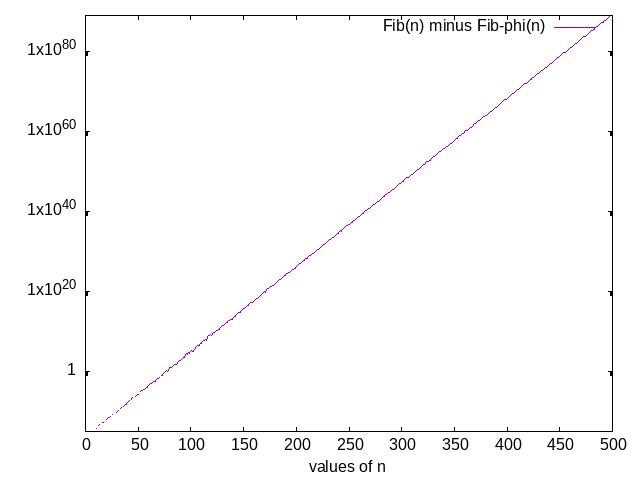
\includegraphics{1-13.png}

\end{document}
